%!TEX root = ../../main.tex


\chapter{Introduction}	\label{ch::introduction}
\chaptermark{SiV Centers}

		\epigraph{``Every competent physicist can \enquote{do} quantum mechanics, but the stories we tell ourselves about what we are doing are as various as the tales of Sheherazade, and almost as implausible.''}{\textup{David J. Griffiths}}

		The International System of Units (SI, abbreviated from the French Syst\`eme international d'unit\'es) emerged in the late $18^{th}$ century as a coherent metric system of measurement with rationally related units and simple rules for combining them \cite{zwinckels::1}. Since its inception it was improved and augmented continuously in an ongoing effort to accommodate continued scientific and technological progress. The current SI system is comprised of seven base units: The kilogram (\SI{}{\kg}), the second (\SI{}{\s}), the Ampere (\SI{}{\ampere}), the Kelvin (\SI{}{\kelvin}), the mole (\SI{}{\mole}) and the candela (\SI{}{\candela}). Currently a redefinition of four of base units (kilogram, mole, Kelvin, Ampere) in terms of fundamental constants is under way \cite{zwinckels::3, Milton, Martin (14 November 2016). Highlights in the work of the BIPM in 2016}. The proposed change will improve the definitions of these base units to make them easier to realize experimentally, particularly for the measurement of electrical quantities \cite{zwinckels::paper}. It will also eliminate the last remaining base unit definition which relies on a historic material artifact, the international prototype of the kilogram. As a result all base units will, for the first time, be tied to one or more fundamental constants of nature.

		As these developments are put into motion, similar discussions regarding the SI base unit for luminous intensity, the candela, have emerged. It has been suggested that it can be improved by leveraging recent advances in classical radiometry and photometry as well as the development of novel quantum devices and techniques \cite{Cheung2007}.

		At the time of writing the definition of the candela read:

		\begin{quote}
			The candela is the luminous intensity, in a given direction, of a source that emits monochromatic radiation of frequency \SI{540d12}{\hertz} and that has a radiant intensity in that direction of $638^{-1} \SI{}{\watt\per\steradian}$.
		\end{quote}

		Traditional applications relying on this definition in conjunction with accurate photometric and radiometric measurements are light design, manufacturing and use of optical sources, detectors, optical components, colored materials and optical radiation measuring equipment \cite{zwinckels::paper}. In the classical regime of optical radiation high flux levels dominate. Here primary optical radiation scales for sources and detectors are generally based on cryogenic radiometry establishing a link to the SI units of electricity \cite{Cheung2007::5}. Other calculable sources such as synchrotron and blackbody radiators can serve as primary source scales in the ultraviolet and deep-UV regions by establishing traceability to SI units of thermometry, electricity and length \cite{zwinckels::paper, Cheung2007}.

		Scaling down to the quantum world of radiometry is associated with a loss of measurement accuracy. In this regime dedicated photon counting techniques are required to deal with the challenge of low flux levels. Since they rely on counting photons directly, in principle they can provide efficient and traceable measurements and improved uncertainties. For high-accuracy absolute radiometry in this regime, predictable single or quasi-single-photon sources and photon detectors as well as associated new quantum-based calibration methods and standards are called for. To promote the development of such technologies a reformulation of the candela has been proposed in terms of \emph{countable} photon units \cite{zwinckels::paper, Cheung2007, Milton, Martin (14 November 2016). Highlights in the work of the BIPM in 2016, www.quantumcandela.org}. Here we emphasize the distinction between \emph{countable} and \emph{calculable} sources of photons. The latter being available as blackbodies or synchrotron radiators.

		A straightforward quantum-based reformulation has been suggested based on \cite{Cheung2007, zwinckels::paper}:

		\begin{equation}
			P = n h \nu,
		\end{equation}

		where the radiant intensity per steradian $P = 638^{-1} \SI{}{\watt\per\steradian}$ in a given direction and the photon frequency $\nu = \SI{540d12}{\hertz}$ are assumed to be exact with their numerical values inherited from the present definition of the candela. The anticipated proposed changes to the SI system will define Planck's constant $h = \SI{6.62607015d-34}{\joule\second}$ as an exact numerical constant \cite{porposal}. As a consequence the number of photons per second per steradian in a candela $n$ becomes a constant defined as:

		\begin{equation}
			n = \frac{P}{h \nu} \approx \SI{4.0919429d15}{\counts\per\second\per\steradian}.
		\end{equation}

	Given this definition of the radiant intensity of a candela in terms of countable photons, a possible formulation of the quantum candela could read:

	\begin{quote}
		The candela is the luminous intensity, in a given direction, of a source that emits photons of frequency \SI{540d12}{\hertz} at a rate of \num{4.0919429d15} photons per second per steradian in that direction.
	\end{quote}

	This definition would incur a deviation of \SI{0.0014}{\percent} from the current value of the candela. This is an acceptable change, taking into account the fact that current experimental realizations of the candela are limited to uncertainties of \SI{0.02}{\percent} \cite{Cheung2007}. Proposals such as this are regularly reviewed by the Consultative Committee for Photometry and Radiometry ensuring that the current best measurement practices and existing as well as emerging needs of the user community of the candela are met \cite{zwinckels::paper}.

	While a proposed formulation of a quantum-candela can be considered a small change to the SI system, a shift towards quantum based radiometric SI units it likely to become a critical enabler driving the development of accurate and traceable measurement methods on the single-photon level. In order for the definition of the quantum-candela to have practical meaning, photon counting detectors are required capable of accurately resolving single-photons. To ensure proper calibration of such devices, reliable deterministic \spss are key. As novel instruments and associated calibration standards emerge, our ability to work with individual photons in a wide range of applications is expected to improve \cite{Rodiek2017::1, Rodiek2017::2, Rodiek2017::3, Rodiek2017::4}. The quest for \spss is supported by large research projects such as ``Single-Photon Sources for Quantum Technology" funded by European Metrology Research Program.

	Advances in radiometry are particularly important for fields like quantum communication and quantum computing. They are heavily reliant on deterministic reliable single-photon sources and well-calibrated detectors. As such they have proven to be major driving forces in their development \cite{vaigu2017::1, vaigu2017::2}. Amongst others, some well known applications include quantum key distribution \cite{janine::12, janine::28, janine::29} or transmission in a quantum network \cite{janine::18, janine::51, janine::54}.

	At present several candidates for on-demand single-photon sources are available, which we shortly mention here. One possibility consists of using a laser beam attenuated such that the mean number of photons in the beam becomes close to one \cite{Vaigu2017::6, Vaigu2017::7, Vaigu2017::8}. However, the mean photon number cannot be controlled perfectly and a non-zero probability remains that multiple photons are present in the beam simultaneously.

	Quasi-single photon states can be realized more efficiently using photon-pairs consisting of a signal and an idler photon. Pairs are created when a photon interacts with a non-linear optical medium in a process called spontaneous parametric down-conversion (SPDC) \cite{Shih, Yanhua (2003). Entangled biphoton source - property and preparation, Vaigu2017::9, Vaigu2017::10, Vaigu2017::11, Vaigu2017::12}. The deciding feature of the process is the strong time-correlation between signal and idler photons. If both photons are injected into individual signal paths, an detection event in one of the paths heralds the existence of a photon in the other path. SPDC pairs can thus be used to construct single-photon sources. Unfortunately, due to the poor efficiency of the SPDC process, the probability of generating pairs is unfavorable \cite{zwinckels::paper, Bock2016}. Thus efforts have been undertaken to improve the efficiency \cite{Bock2016, zwinckels::112, zwinckels::113}.

	Quantum dots emit photons by recombination of electron-hole pairs created by optical excitation or via an electric current \cite{zwinckels::115, Vaigu2017::18, Vaigu2017::15}. The choice of semi-conducting material determines the electronic structure of the system and thus the characteristics of the emitter. Similarly, single-photons can be obtained as a result of radiative transitions between energy levels of single atoms or molecules trapped in an optical cavity \cite{zwickels::116}. While these sources have desirable properties such as high-collection efficiency, the practical usefulness is limited due to being technologically demanding. Amongst others a high vacuum is needed to operate these sources \cite{zwickels::paper}.

	For a wide range of \spss, significant progress has been made towards improving purity, indistinguishably and collection efficiency \cite{Vaigu2017::21, Vaigu2017::22, Vaigu2017::23, Vaigu2017::24, Vaigu2017::25}.

	As it stands, a \sps suitable for the calibration of single-photon detectors remains difficult to realize \cite{Vaigu2017::paper}. Ideally, a standard \sps should be emitting with a quantum efficiency of \SI{100}{\percent} indicating that the entire excitation energy is transformed into radiation without losses. At the same time single photons should be emitted with a probability of one and subsequently collected with perfect efficiency.

	Very recently, another interesting direction has been explored, identifying \ccs in \nds involving silicon \cite{Rodiek2017::12, Rodiek2017::13} and nitrogen \cite{Rodiek2017::8} as promising candidates for the realization of standard \spss \cite{Rodiek2017,Vaigu2017}. In particular it was shown that it is possible to absolutely calibrate \spss using a classical detector and a calibrated spectrometer, establishing an unbroken traceability chain to the SI system. The photon flux of the source can be controlled via the settings of the pump laser repetition rate. In this way a direct link between the high photon flux levels of the classical regime and low photon flux levels in the quantum world has been formed. For the nitrogen vacancy center a photon flux rate of $\approx \num{1.4d5}$ photons per second was recorded.

	In this thesis we continue researching the potential of \ccs in diamond as \spss. More precisely, we focus on the \sivc. In doing so we aim to add momentum to the development of \sps as high-accuracy calibration devices and subsequently, to the development of photon counting detectors and the adoption of the quantum-candela.

	The \siv in diamond is an ideal candidate for single photon calibration purposes. It is a very efficient and stable narrow \lw emitter, producing single photons with high intensity. Conveniently, \sivs operate at room temperature under normal pressure and hence do not require overly sophisticated experimental setups. As an alternative to hosting \sivs in bulk diamond, they can be implanted in nano-sized diamond grains offering increased collection efficiency. Grains containing individual \sivs can be identified and preselected according to their properties.

	
	In this thesis we synthesize \nds with \sivs using a variety of different techniques. \Cvd, \hpht synthesis as well as wet-milling methods are used to produce a sizable set of samples. To investigate the samples, i.e.\ to study the optical properties of embedded \sivs we rely on optical excitation. In particular, confocal microscopy is used to collect emitted fluorescent single-photons. An attached spectrometer or a \HBT setup offer further insights into the properties of the \siv as a \sps. 


   	Our work can roughly be subdivided into two larger explorations. The first revolves around charting the luminescence properties of a large set of \nds and their hosted emitters, allowing us to establish distributions of selected \siv properties. To our knowledge, our efforts result in the largest coherent examination of \sivs in \nds to date. In contrast to that the second exploration focuses on individual \nds and our attempts to relocate them to different nano structures in order to achieve a coupling between \sivs and the host structure. First we attempt to realize a controllable hybrid-integrated \sps by placing a \nd containing \sivs on top of a \vcsel (\VCSEL). Furthermore, we combine \nds with plasmonic nano-antennas in order to enhance the emission properties of the contained \sivs. 
   	To this aim, a range of samples were investigated in the search for well-suited \nds hosting single \sivs (\cref{fig::milky_way1}).

   	\begin{figure}[htbp]
   		\centering
   		\begin{tikzpicture}
   			\begin{scope}[spy using outlines={rectangle,blue,magnification=3,size=2.5cm}]
   			\node{\testbox{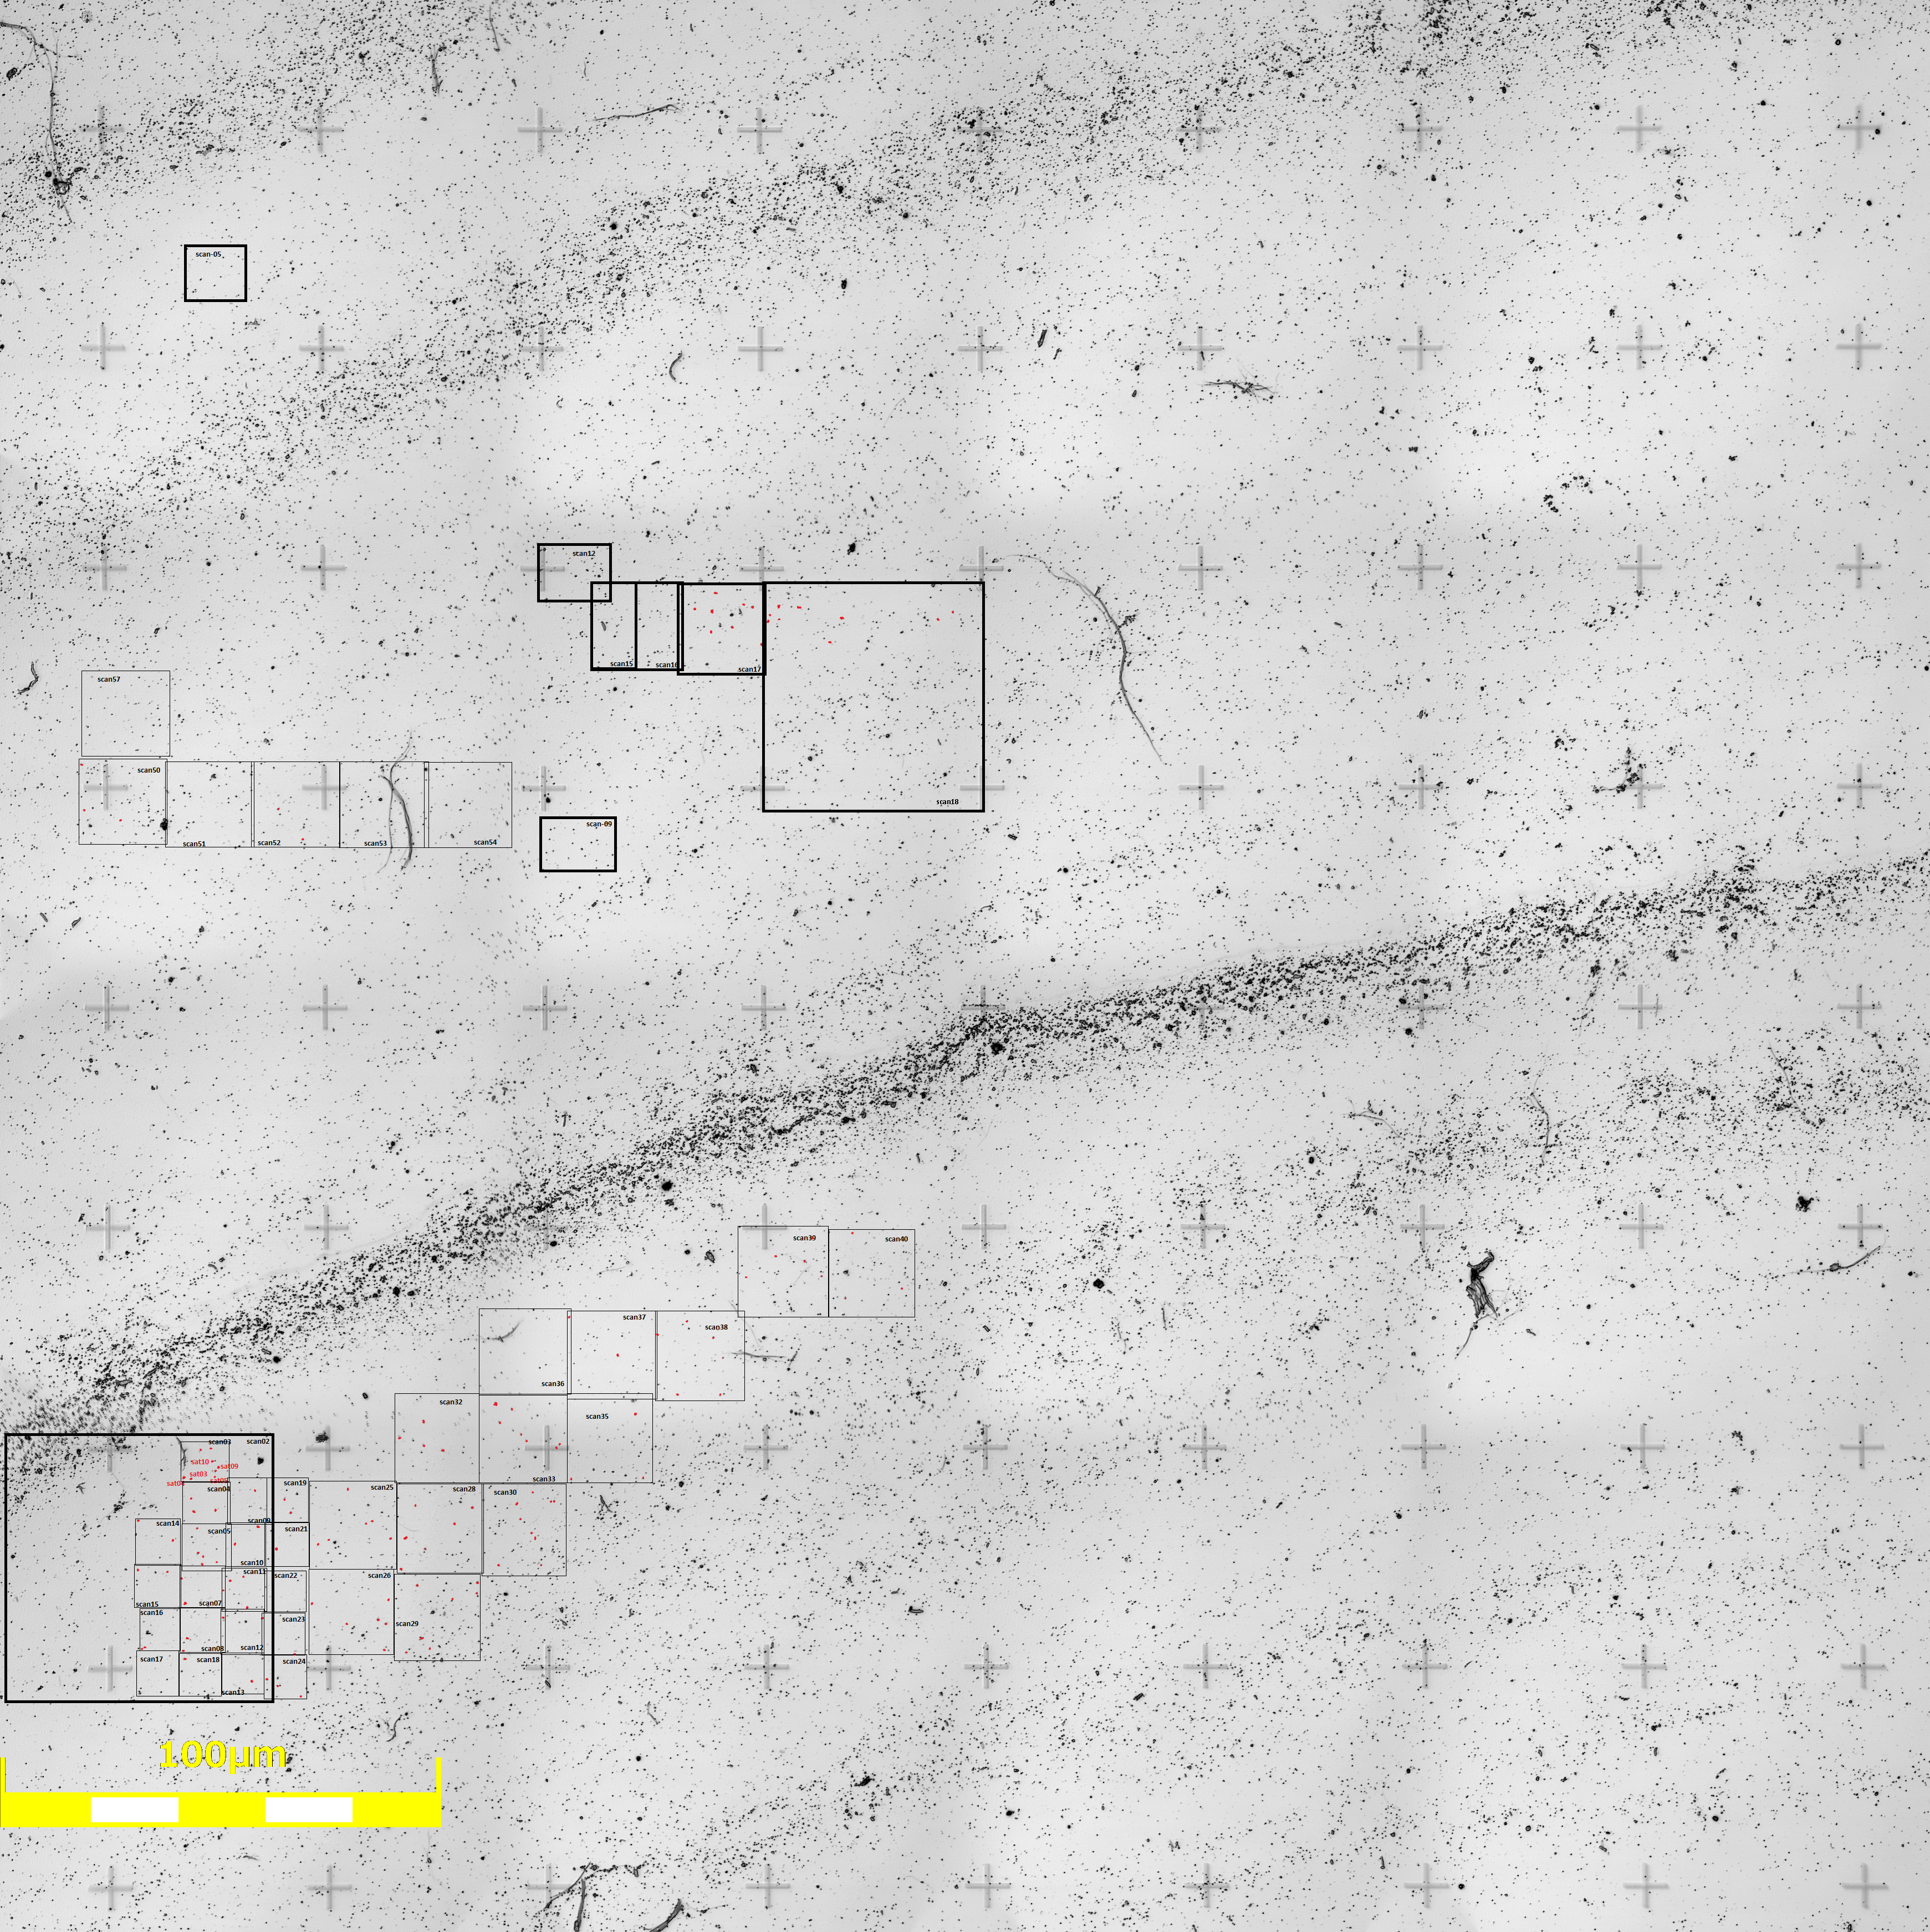
\includegraphics[trim = 0 0 0 0,  clip= true, width = \linewidth]{./pics/M02-16_structure2_paint.png}}};
   			\spy on (-6,-4.8) in node (a) [left] at (0,-6);
   			\end{scope}
   		\end{tikzpicture}
   		\caption[LSM scan, overview of a $\SI{0.5}{mm}\times\SI{0.5}{mm}$ area]{Sample surface of a $\SI{0.5}{mm}\times\SI{0.5}{mm}$ area of one of the investigated samples in search for suitable \nds. Black frames correspond to areas of which confocal scans were recorded to identify \nds emitting \fl. Red colored dots indicate \nds which are isolated enough for the \pp process and of which at least a \pl spectrum and a saturation measurement and in some cases a \gt measurement were recorded. The inset shows a magnification of the area framed in blue for better visibility of the red colored dots.}
   		\label{fig::milky_way1}
   	\end{figure}


	The thesis is structured as follows: \cref{ch::sivs} introduces the reader to \ccs and diamond as a host material. A discussion of \sivs restricted to their most important luminous properties is presented. \cref{ch::pl_setup} familiarizes the reader with the essential experimental setup and methods deployed in this thesis to study \siv luminescence. Various relevant methods of synthesizing sample \nds containing \sivs are presented and discussed in \cref{ch::fabrication_nanodiamonds}. \cref{ch::crystal_quality} is dedicated to the important topic of gauging the quality of fabricated samples. The results of charting the luminous properties of our \nds samples is presented in \cref{ch::distribution}. Our attempts of coupling \nds hosting \sivs to two different nano structures is investigated in \cref{ch::coupling}. Finally we summarize and discuss the findings of this thesis in \cref{ch::conclusion}.
